\input{../slides-common/preambule}

\pdsetup{
   lf = {\cursopequeno},
   cf = {\theslide},
   rf = {Introdução}, palette = {\palette}, randomdots={false}
}


%opening
\title{\cursogrande\\ \vspace{1cm}Introdução}

\begin{document}
   \maketitle[randomdots={false}]
   
   \begin{slide}{Agenda}
      \tableofcontents[content=sections]
   \end{slide}

\section[ slide = true]{Motivação}
\begin{slide}[toc=]{Motivação}
\begin{itemize}
	\item ``Os alunos precisam entender arquitetura de computador a fim de \textcolor{red}{fazer melhor uso das ferramentas de software e linguagens de programação que eles usam para criar programas}. Estudantes também devem compreender os compromissos complexos entre velocidade de clock de uma CPU, tamanho da memória cache, organização de barramento, número de núcleos do processador e assim por diante.''\\ {(\textit{IEEE/ACM Computer Science Curriculum 2008})}
     
  \item ``Arquitetura de computador é um \textcolor{red}{componente chave} da engenharia da computação(...) e o engenheiro da computação atuante deve ter um entendimento prático sobre esse tópico'' \\{(\textit{Computer Engineering 2004 Curriculum Guidelines})}
  \item Sistemas computacionais modernos são \textcolor{red}{máquinas complicadas}
  \item Há \textcolor{red}{muitas soluções} disponíveis
  \item O compromisso \textcolor{red}{\textit{custo-benefício}} sempre está presente
\end{itemize}
\end{slide}

\section[ slide = true]{Objetivos e situações}
\begin{slide}[toc=]{Objetivos e situações de aplicação}
\begin{itemize}
  \item Objetivos do estudo:
  \begin{itemize}
    \item Apresentar os elementos constituintes, suas características e interações, de computadores modernos
  \end{itemize}
  \item Situações de aplicação:
  \begin{itemize}
    \item Projeto e utilização de sistemas computacionais
    \item Análise crítica para seleção de tecnologias
  \end{itemize}
\end{itemize}
\end{slide}

\section[ slide = true]{Arquitetura vs. Organização}
\begin{slide}[toc=]{Arquitetura vs. Organização}
	\begin{itemize}
		\item Arquitetura
   \begin{itemize}
	   \item \textcolor{red}{Atributos do sistema visíveis ao programador}%, com impacto direto na execução lógica de um programa}
         \begin{itemize}
            \item Conjunto de instruções
            \item Número de bits para representar dados
            \item Mecanismos de entrada e saída
            \item Estratégias de endereçamento
         \end{itemize}
   \end{itemize}
			\item Organização
%\end{slide}

%\section[ slide = false ]{Organização}
%\begin{slide}[toc=]{Organização}
   \begin{itemize}
         \item \textcolor{red}{Unidades operacionais e suas interconexões que implementam especificações de uma arquitetura}
         \begin{itemize}
            \item Sinais de controle  
            \item Interface entre computador e periféricos
            \item Tecnologia de memória
            \item Padrão de barramento
         \end{itemize}
    \end{itemize}
	\item Exemplo: disponibilidade de \textcolor{red}{instrução de multiplicação}
    \end{itemize}
\end{slide}

\section[ slide = true]{Sistema hierárquico}
\begin{slide}[toc=]{Sistema hierárquico}
   \begin{itemize}
         \item Conjunto de subsistemas inter-relacionados
         \item Estrutura: modo de inter-relação
         \item Função: operação de cada componente na estrutura
         %\item Padrão de barramento
   \end{itemize}
\end{slide}

\section[ slide = true]{Visão funcional}
 \begin{slide}[toc=]{Visão funcional}
    \begin{figure}[h]
      \centering
      \includegraphics[width = 0.9\textwidth]{figs/f1-1.eps}
    \end{figure}
\end{slide}

%\begin{slide}[toc=]{Operações possíveis}
%    \begin{itemize}
%       \item Operações possíveis: movimentação de dados
%       \begin{figure}[h]
%      \centering
%      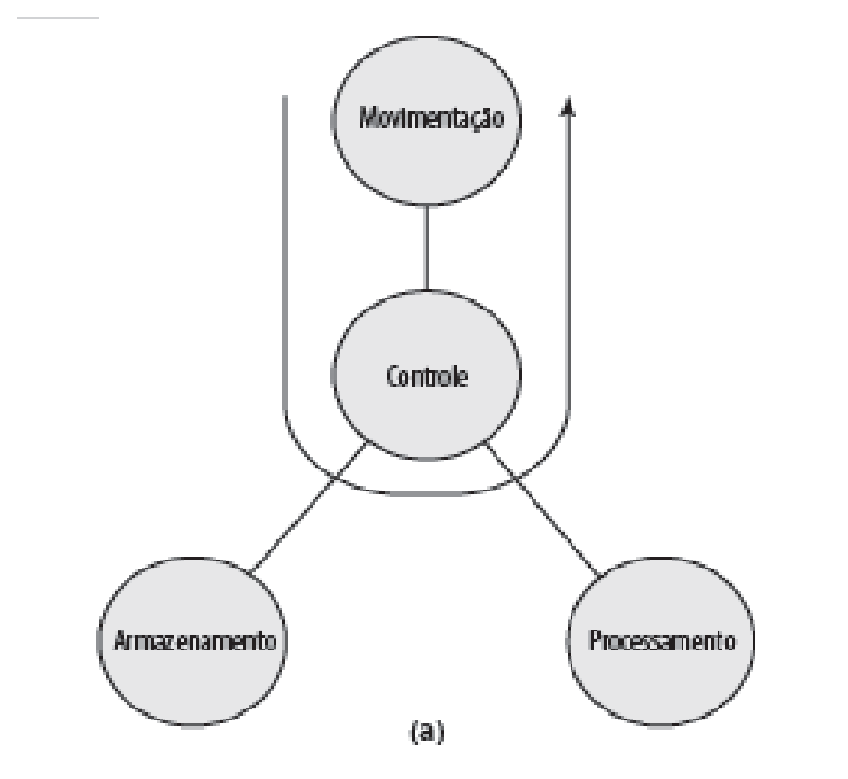
\includegraphics[height = 0.65\textheight]{figs/f1-2a.eps}
%    \end{figure}
%    \end{itemize}
% \end{slide}
%
%\begin{slide}[toc=]{Operações possíveis}
%    \begin{itemize}
%       \item Operações possíveis: movimentação e armazenamento de dados
%       \begin{figure}[h]
%      \centering
%      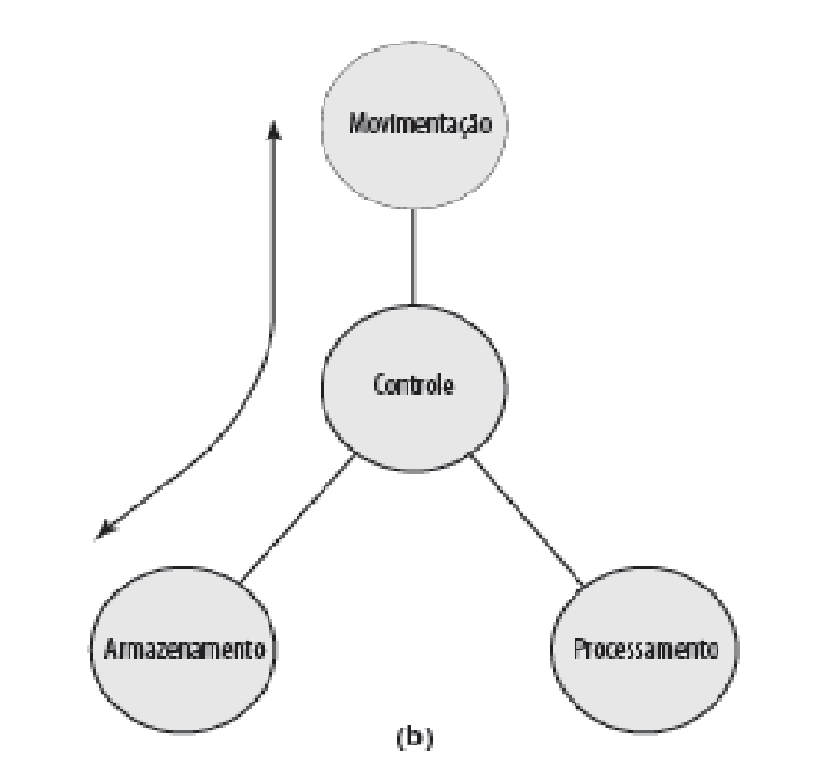
\includegraphics[height = 0.55\textheight]{figs/f1-2b.eps}
%    \end{figure}
%    \end{itemize}
% \end{slide}
% 
%\begin{slide}[toc=]{Operações possíveis}
%    \begin{itemize}
%       \item Operações possíveis: armazenamento e processamento de dados
%       \begin{figure}[h]
%      \centering
%      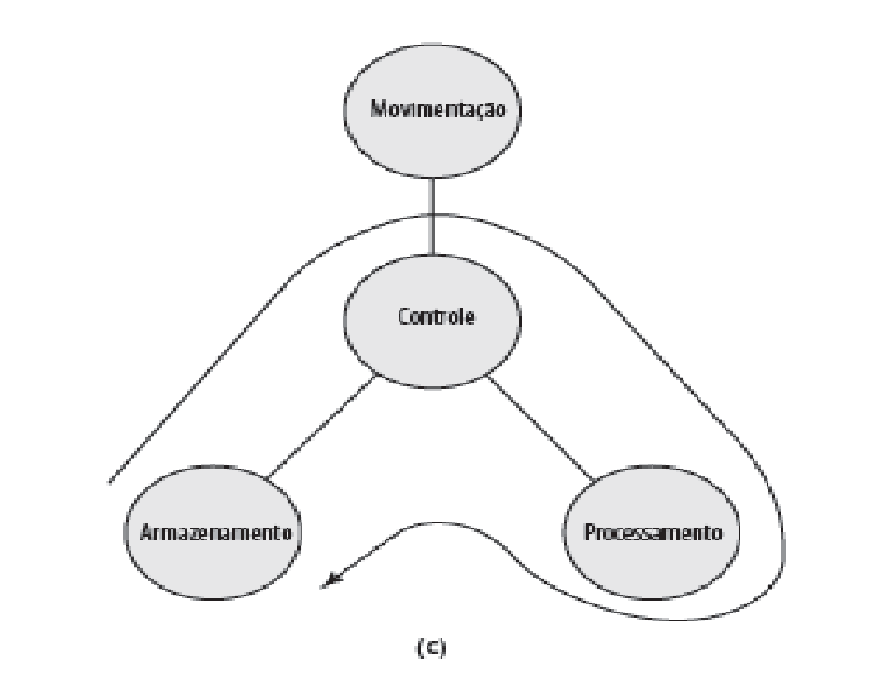
\includegraphics[height = 0.55\textheight]{figs/f1-2d.eps}
%    \end{figure}
%    \end{itemize}
% \end{slide}
%\begin{slide}{Operações possíveis}
%    \begin{itemize}
%       \item Operações possíveis: movimentação, armazenamento e processamento de dados
%       \begin{figure}[h]
%      \centering
%      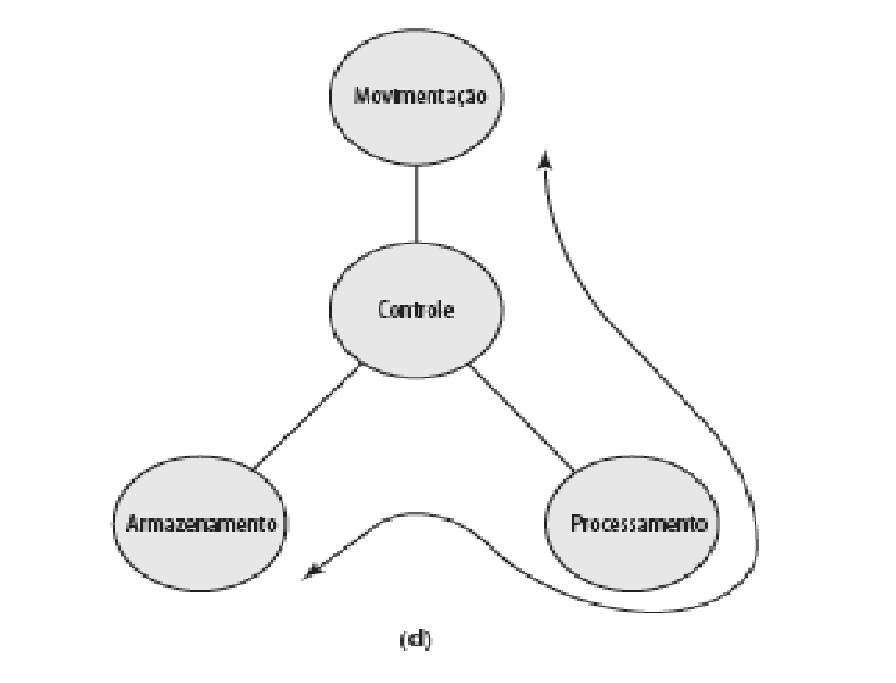
\includegraphics[height = 0.55\textheight]{figs/f1-2c.eps}
%    \end{figure}
%    \end{itemize}
% \end{slide}
% 
 \section[ slide = true]{Visão estrutural}
% \begin{slide}[toc=]{Estrutura: visão geral}
%    \begin{figure}[h]
%      \centering
%      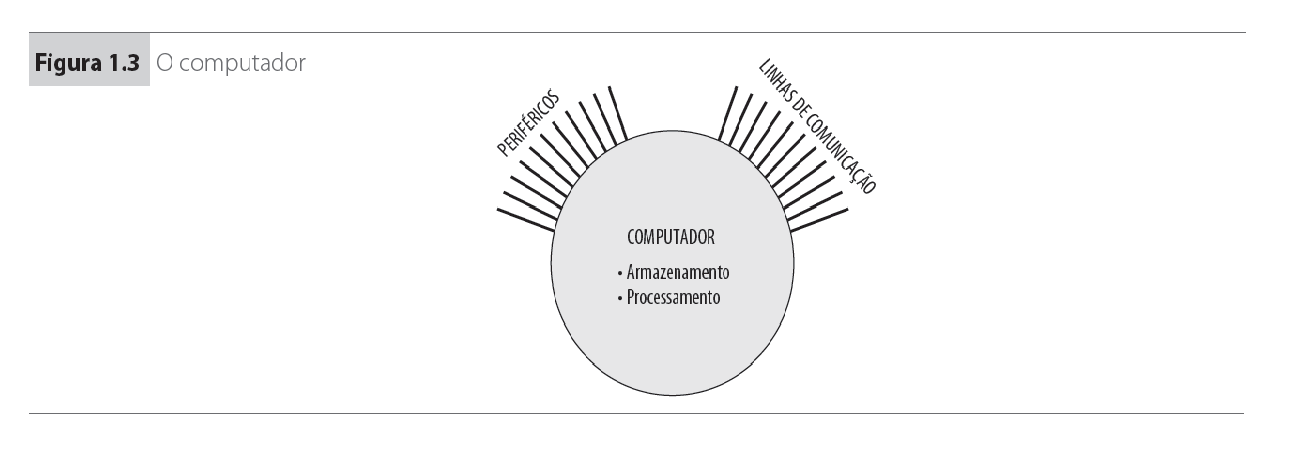
\includegraphics[width = 0.9\textwidth]{figs/f1-3.eps}
%    \end{figure}
% \end{slide}
 
 \begin{slide}[toc=]{Estrutura: sistema hierárquico}
    Em sistemas computacionais em geral
    \begin{figure}[h]
      \centering
      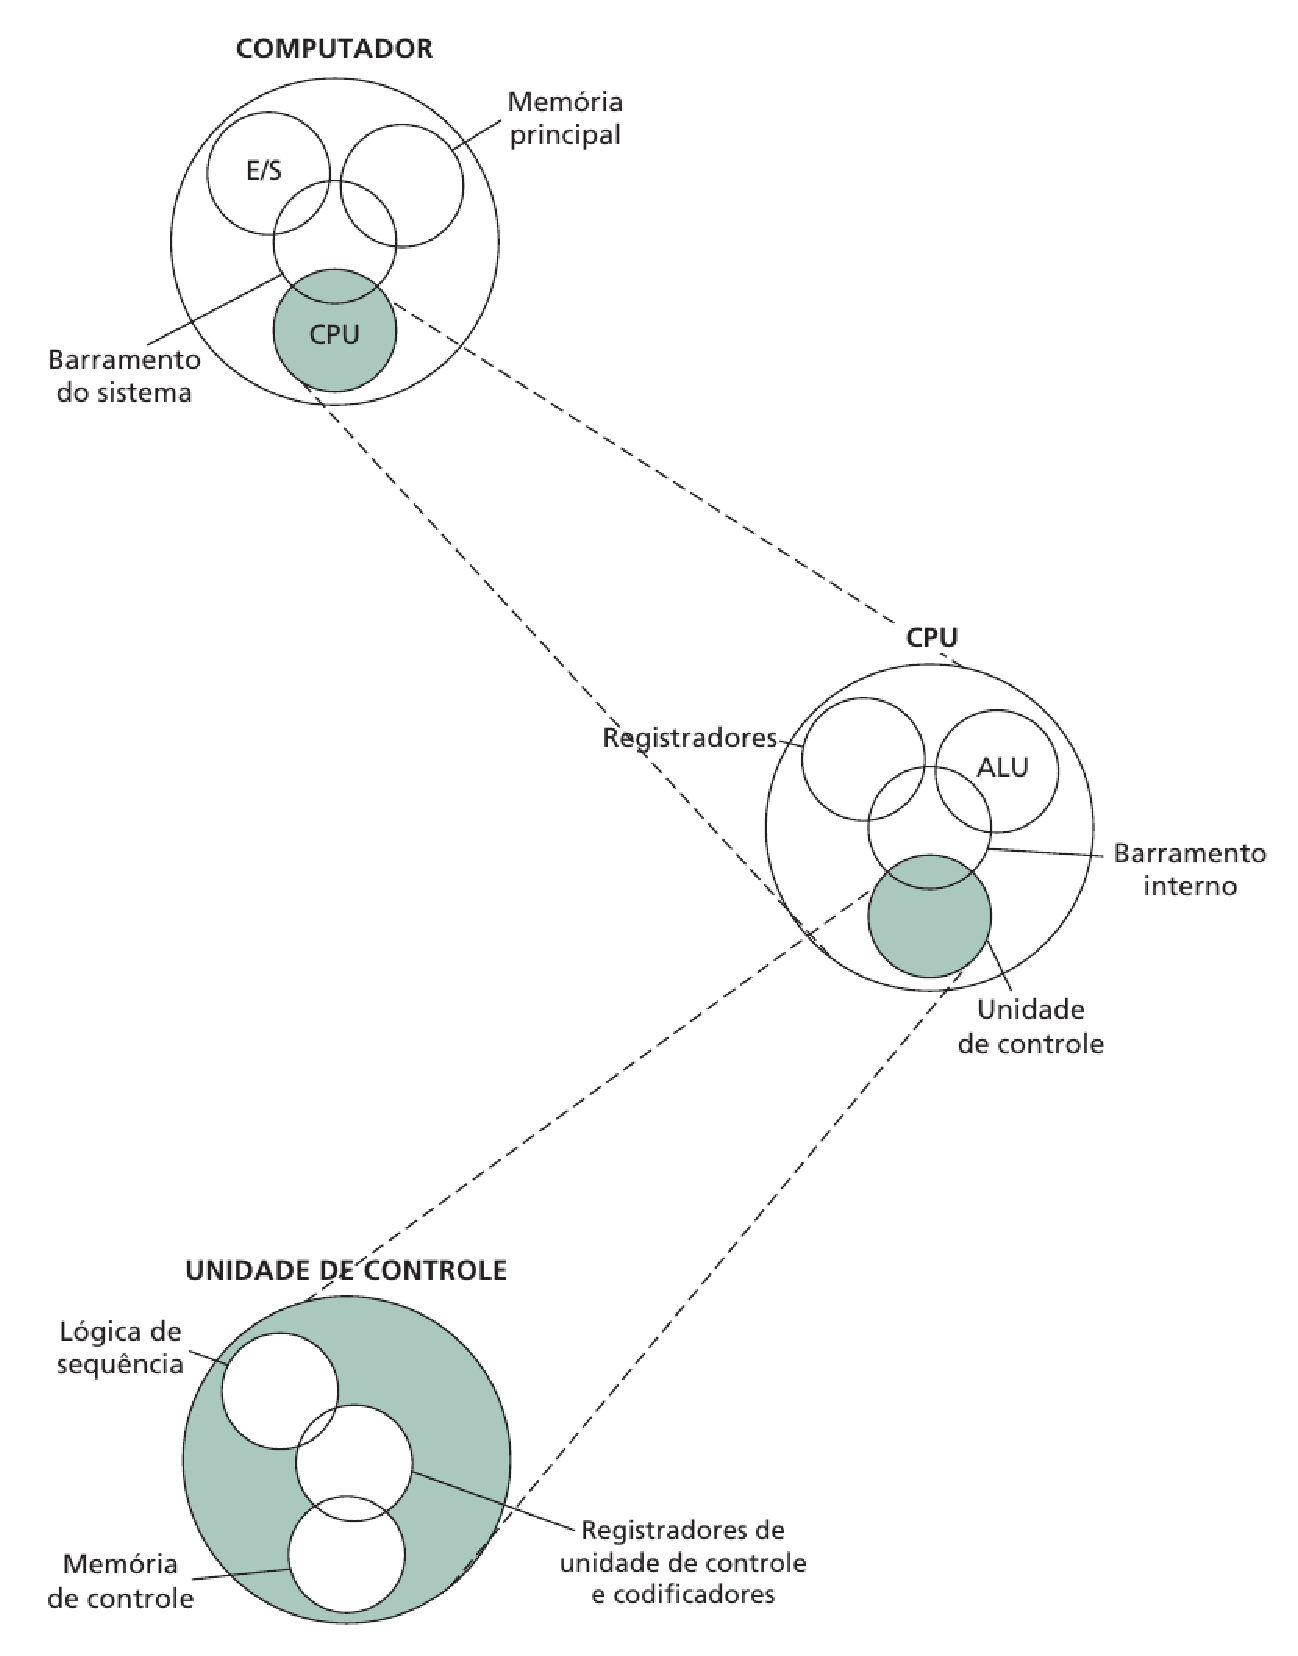
\includegraphics[height = 0.73\textheight]{figs/estrutura.eps}
    \end{figure}
\end{slide}
 
\begin{slide}[toc=]{Estrutura: sistema hierárquico}
    Em um computador multicore
    \begin{figure}[h]
      \centering
      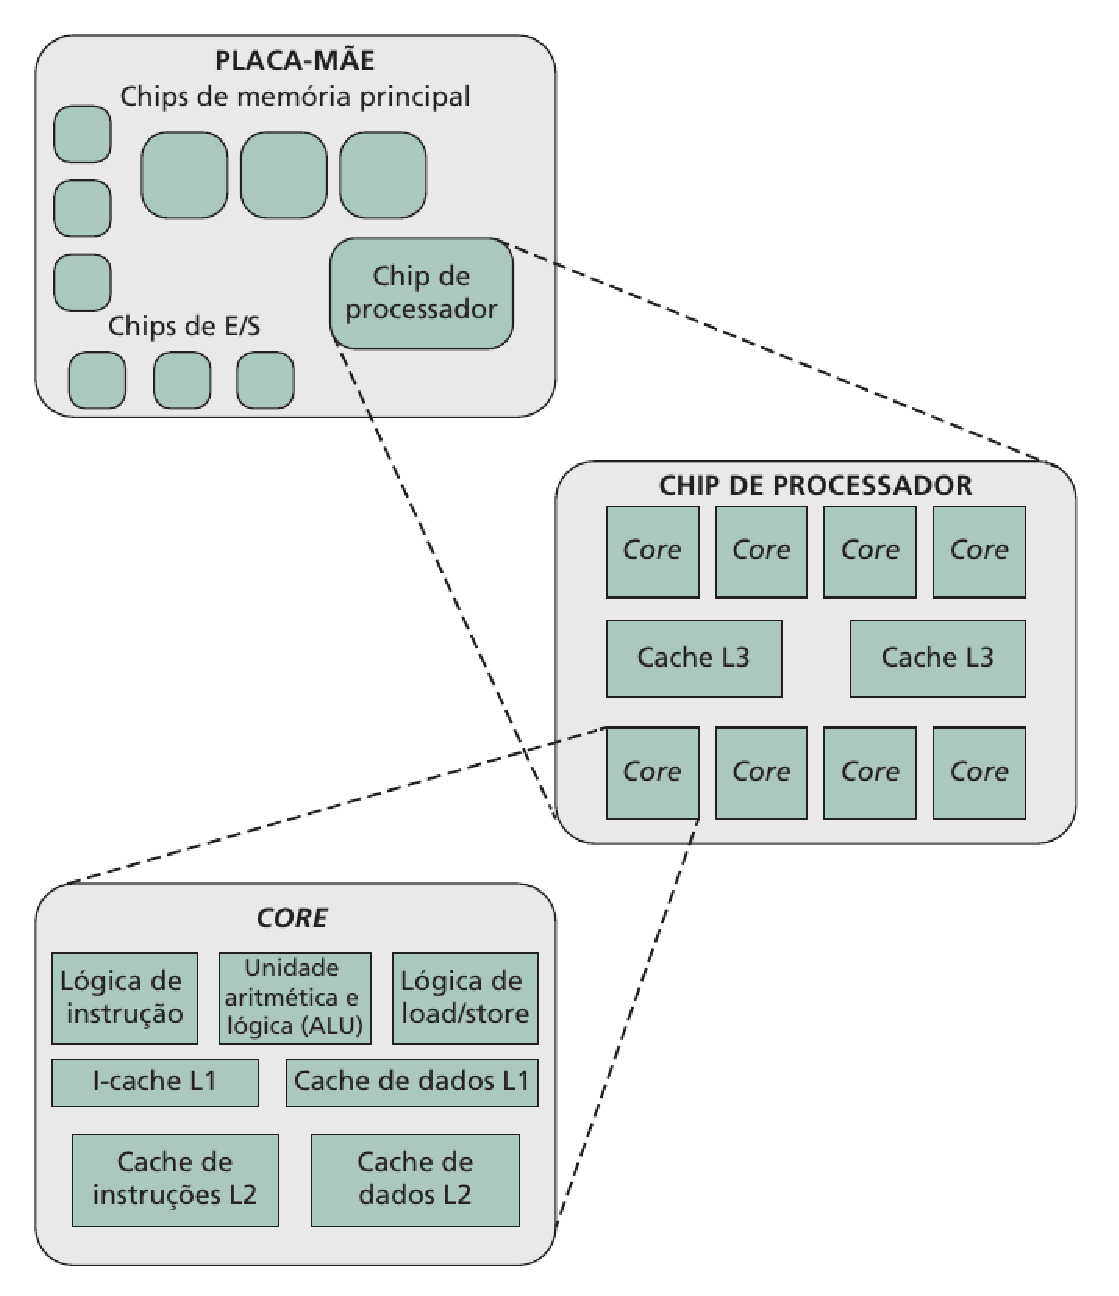
\includegraphics[height = 0.73\textheight]{figs/estrutura_multicore.eps}
    \end{figure}
\end{slide}
 
\begin{slide}[toc=]{Estrutura: sistema hierárquico}
	Chip zEnterprise EC12 (2013)
    \begin{figure}[h]
      \centering
      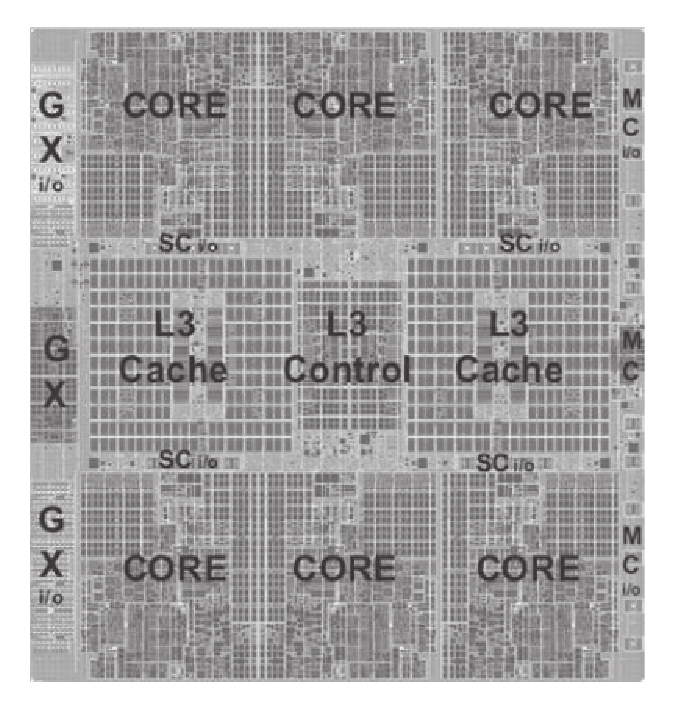
\includegraphics[height = 0.73\textheight]{figs/EC12.eps}
    \end{figure}
\end{slide}

\begin{slide}[toc=]{Estrutura: sistema hierárquico}
	Layout do core do zEnterprise EC12 (2013)
    \begin{figure}[h]
      \centering
      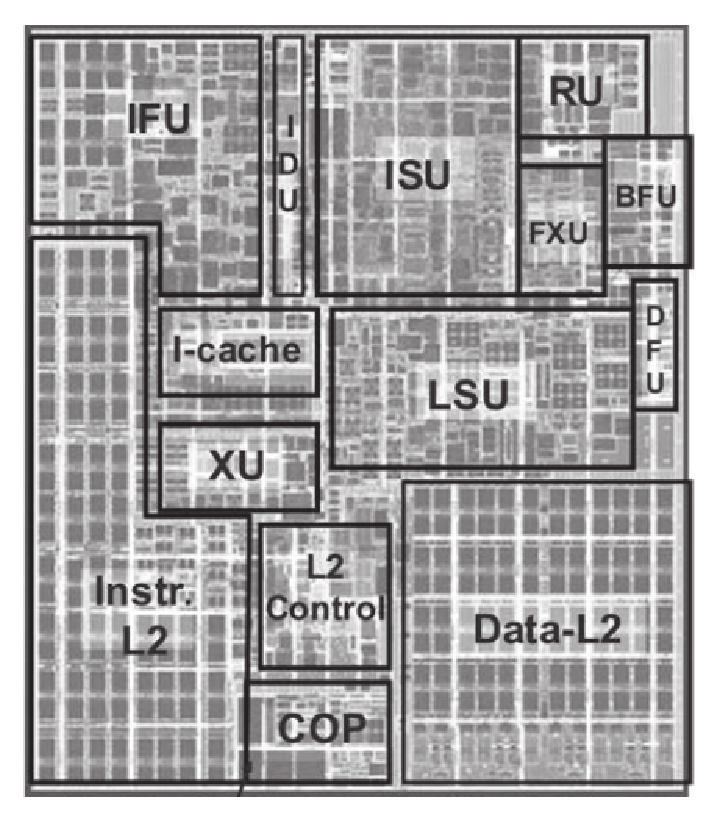
\includegraphics[height = 0.73\textheight]{figs/layout_EC12.eps}
    \end{figure}
\end{slide}

\end{document}
